% !TeX root = main.tex
\chapterimage{chapter-03-algoritmi-quotidiani.jpg}
\chapter{Algoritmi quotidiani}\label{algoritmi-quotidiani}

In questo capitolo proponiamo attività didattiche per una lettura algoritmica di molte delle attività che facciamo ogni giorno e che seguono una sequenza di passi. Infatti, per vestirci, cucinare o realizzare un modello con i mattoncini LEGO®, compiamo azioni che, se osservate dall'esterno, assomigliano molto a un algoritmo. Esploreremo come descrivere algoritmi relativi ad attività quotidiane in modo chiaro, preciso e non ambiguo, mettendo in luce come ciò che per chi descrive sembri ``ovvio'' possa essere interpretato in modi diversi da chi ascolta.

Dal punto di vista informatico, quando un algoritmo viene espresso in un linguaggio che il computer può ``capire'', viene chiamato \textbf{programma}. Il computer esegue il programma solo quando glielo ``chiediamo''. Il computer eseguirà solo ciò che è stato scritto, alla lettera e passo dopo passo, senza intuire o indovinare ciò che non è stato esplicitato e senza fare domande intermedie. Se durante o al termine dell'esecuzione qualcosa non ha funzionato, il programmatore, attraverso la pratica del debugging (vedi~\ref{debug}), potrà esaminare il comportamento dell'esecutore, individuare l'errore e modificare la sequenza.

Le attività di questa sezione propongono alcuni esempi di pratiche didattiche che incarnano le idee mostrate nei video del Capitolo~\ref{capitolo-1-introduzione} (sezione~\ref{pensiero-computazionale}), cioè la sfida del video \emph{Exact Instructions Challenge} per il panino con il burro di arachidi e il video del maestro Manzi sul lavarsi i denti. Potrete poi sbizzarrirvi nel progettare molte altre attività simili declinandole nel modo più opportuno alle vostre classi e scegliendo ambientazioni che diano significato e motivazione (ad esempio le regole di un gioco motorio, un laboratorio artistico, una storia inventata da alunni e alunne).

\section{Traguardi e obiettivi generali }\label{traguardi-e-obiettivi-generali}

\begin{itemize}
\item
  Scomporre un compito complesso in una sequenza di istruzioni elementari e ben definite.
\item
  Ordinare le istruzioni in modo coerente.
\item
  Utilizzare un linguaggio chiaro, preciso e non ambiguo per descrivere istruzioni.
\item
  Immedesimarsi nel punto di vista dell'esecutore, anticipando possibili fraintendimenti.
\item
  Riconoscere e correggere ambiguità nelle istruzioni.
\item
  Attuare pratiche di debugging.
\item
  Progettare e utilizzare un linguaggio condiviso per descrivere azioni.
\end{itemize}

\section{Prerequisiti }\label{prerequisiti}

Le attività proposte non richiedono particolari conoscenze informatiche pregresse: è sufficiente che alunni e alunne sappiano seguire e dare istruzioni in linguaggio naturale e ordinare nel tempo le fasi di una storia o di un'azione quotidiana. Per l'Attività 3 è utile che abbiano già incontrato le principali forme geometriche e abbiano avuto qualche esperienza di composizione con figure usando costruzioni di vario tipo.

Alcune attività sono progettate per essere proposte a chi non ha ancora raggiunto un livello di apprendimento della letto-scrittura adeguato ma, una volta che tali abilità strumentali saranno acquisite, sarà possibile proporre richieste più articolate e sfidanti.

\section{Contenuti, in breve }\label{contenuti-in-breve}

Questo capitolo contiene attività pensate per capire cosa significhi sviluppare una lettura algoritmica di un compito: scomporlo in istruzioni essenziali, metterle in ordine e formularle con precisione. Riprendendo quanto visto nel Capitolo~\ref{fondamentali-di-informatica} sulle istruzioni, vedremo come:

\begin{itemize}
\item
  definire le \textbf{istruzioni} elementari per raggiungere un certo obiettivo;
\item
  stabilire la \textbf{sequenza} corretta di istruzioni, cioè come ordinarle per ottenere un certo effetto;
\item
  \textbf{esprimere le istruzioni} in modo chiaro e non ambiguo.
\end{itemize}

\textbf{Attività 1 -- Sequenze e ordine}: alunni e alunne scompongono azioni o storie in istruzioni elementari, le mettono in sequenza e sperimentano cosa cambia (o non cambia) quando si altera l'ordine, per capire perché in un algoritmo l'ordine delle istruzioni è fondamentale, e talvolta sequenze diverse possono produrre lo stesso risultato.

\textbf{Attività 2 -- Istruzioni e programmi}: attraverso la richiesta di eseguire programmi dati e poi di inventarne di nuovi si introduce l'idea di \emph{Manuale delle istruzioni} che definisce ``quali istruzioni esistono e che cosa fanno''.

\textbf{Attività 3 -- Descrivere configurazioni geometriche}: far ricostruire una configurazione geometrica a un esecutore umano che segue le istruzioni alla lettera (senza interpretare né fare domande) e migliorare iterativamente le descrizioni tramite debugging, per arrivare a un linguaggio condiviso e rigoroso.

\section{Modalità di lavoro }\label{modalituxe0-di-lavoro}

Tutte le attività che seguono possono essere svolte in classe.

\begin{itemize}
\item
  Si alterneranno fasi di lavoro a coppie con momenti di confronto collettivo o a piccoli gruppi.
\item
  Lo spazio deve permettere di lavorare a coppie in modo che i membri di ciascuna coppia possano comunicare tra loro agevolmente.
\item
  Sarà importante osservare lo svolgimento delle varie attività tenendo traccia delle parole e delle produzioni di alunni e alunne (ad esempio, fornendo schede strutturate per scrivere o disegnare, ma anche scattando foto alle loro produzioni) da usare a supporto di discussioni collettive.
\end{itemize}

In tutte le proposte è cruciale mantenere netta la distinzione tra i ruoli di programmatore ed esecutore. Il \textbf{programmatore} \guideiconProgrammatore\ ha il compito di progettare e scrivere l'intera sequenza di istruzioni prima dell'esecuzione, cercando di prevedere come verranno interpretate. L'\textbf{esecutore} \guideiconEsecutore, invece, deve limitarsi a seguire le istruzioni alla lettera, senza ``aggiustare'' ciò che non è stato specificato e senza introdurre interpretazioni personali.

Questa distinzione rende visibile un'idea chiave: l'output di un programma non è ``l'intenzione'' di chi lo ha scritto, ma ciò che è effettivamente espresso nelle istruzioni disponibili e nel loro ordine.

Un ulteriore punto di attenzione riguarda il modo in cui le istruzioni vengono formulate: il linguaggio naturale è intrinsecamente ambiguo e dipende dal contesto, dalle conoscenze e dalle inferenze di chi ascolta o legge. Proprio per questo, molte attività mirano a far emergere ambiguità tipiche (``quanto?'', ``dove?'', ``rispetto a cosa?'', ``con quale orientamento?'') e a costruire progressivamente convenzioni condivise (ad esempio un \emph{manuale delle istruzioni}, introdotto in~\ref{manuale-delle-istruzioni}, o un lessico comune per descrivere posizioni e relazioni tra figure). Questo passaggio prepara il terreno per comprendere perché in informatica si introducono \textbf{linguaggi formali}: essi non eliminano la complessità del problema, ma rendono esplicite le regole di scrittura e di interpretazione, così che la stessa istruzione, nello stesso contesto formale, venga interpretata dall'esecutore in modo sempre uguale e prevedibile.

\section{Attività 1: sequenze e ordine}

Come abbiamo visto nel Capitolo~\ref{fondamentali-di-informatica}, le istruzioni date a un elaboratore vengono eseguite in sequenza e cambiarne l'ordine produce, in generale, risultati diversi. Quindi, sarà importante proporre attività in cui alunni e alunne possano riflettere sull'importanza di seguire o rispettare un ordine preciso quando, ad esempio, si scompongono attività quotidiane o storie in una sequenza di momenti.

\subsection{Preparazione}

\begin{itemize}
\item
  Stampare e ritagliare diverse immagini che raffigurano momenti di un'attività o scene di una storia.
\item
  Munirsi di post-it (per disegnare o scrivere istruzioni, numeri, parole chiave).
\end{itemize}

\subsection{Descrizione di proposte didattiche }\label{descrizione-di-proposte-didattiche}

\subsubsection{Riordinare delle immagini date}
\ruoliattivita{\ruoloProgrammatore}

In questo tipo di proposta a ciascuno viene consegnato un insieme di carte che raffigurano i diversi passi da fare per raggiungere un dato obiettivo (ad esempio avere i denti puliti, avere lo zaino pronto, andare a scuola) o di una storia. Le carte vengono inizialmente consegnate non ordinate e la richiesta è quella di metterle in ordine, anche eventualmente numerando i vari passi.

\subsubsection{Disegnare immagini o scrivere istruzioni in ordine}
\ruoliattivita{\ruoloProgrammatore}

In questo tipo di proposta a ciascuno viene chiesto di scegliere una storia che conosce o un'attività, suddividerla in momenti ordinati e poi descrivere ciascun momento con un'immagine o un breve testo (ad esempio su singoli foglietti o post-it da disporre in sequenza).

\subsubsection{Cambiare l'ordine e studiarne gli effetti}
\ruoliattivita{\ruoloProgrammatore\quad\ruoloEsecutore}


In questo tipo di proposta a ciascuno viene richiesto di esplorare cosa accade cambiando l'ordine delle istruzioni di una sequenza data. 

Sarà importante proporre anche situazioni in cui l'ordine di alcune
istruzioni può essere scambiato senza modificare il risultato finale.

Consideriamo, ad esempio, l'azione di preparare lo zaino. Una possibile sequenza consiste nell'\textbf{aprire lo zaino}, \textbf{prendere i libri}, \textbf{mettere i libri nello zaino} e infine \textbf{chiudere lo zaino}.

\begin{figure}[htbp]
    \centering
    
\includegraphics[width=0.95\linewidth]{img/cap3-sequenza1.png}
    % \caption{Una possibile sequenza di azioni per preparare lo zaino.}
    % \label{fig:cap3-sequenza1}
\end{figure}

Le prime due azioni, tuttavia, possono essere eseguite anche nell'ordine inverso: si possono prima \textbf{prendere i libri} e poi
\textbf{aprire lo zaino}, proseguendo quindi nello stesso modo.

\begin{figure}[htbp]
    \centering
    
\includegraphics[width=0.95\linewidth]{img/cap3-sequenza2.png}
    % \caption{Una sequenza alternativa che produce lo stesso risultato.}
    % \label{fig:cap3-sequenza2}
\end{figure}

Il risultato non cambia, perché queste due azioni sono indipendenti
l'una dall'altra. Non tutte le azioni della sequenza possono però essere scambiate liberamente: per esempio, è necessario aprire lo zaino prima di inserirvi i libri e chiuderlo solo dopo averli inseriti.

Il confronto tra le due sequenze permette quindi di introdurre, in modo intuitivo, l'idea che alcune istruzioni possono essere scambiate senza effetti sul risultato, mentre tra altre esistono vincoli di precedenza.

\subsubsection{Inventare storie ``buffe''}
\ruoliattivita{\ruoloProgrammatore\quad\ruoloEsecutore}

Oltre a trovare la sequenza corretta, si può proporre una variante creativa: inventare ``storie buffe'' mescolando l'ordine delle scene. In questo caso, la sequenza prodotta diventa un dispositivo narrativo, un artefatto da raccontare, disegnare o persino mettere in scena. Gli errori o le sequenze ``sbagliate'' diventano risorsa: come suggerisce Rodari nella sua \emph{Grammatica della fantasia}, l'ordine alterato può generare narrazioni impreviste e divertenti, insegnando a ``smontare e rimontare'' le storie come fossero costruzioni.

\subsection{Contenuto informatico }\label{contenuto-informatico}

In informatica, la \textbf{sequenza di istruzioni} è la struttura di base (vedi~\ref{elementi-comuni}) su cui si costruisce ogni programma. Prima di introdurre concetti più complessi come le \textbf{selezioni} (\emph{se-allora}) o le \textbf{ripetizioni} (\emph{ripeti}), è essenziale che alunni e alunne comprendano a fondo cosa significhi eseguire azioni in un ordine preciso e senza ambiguità.

Le attività descritte permettono di lavorare su alcune idee chiave:
\begin{itemize}
\item
  Ogni azione deve essere descritta in modo esplicito, senza sottintesi;
\item
  L'ordine conta: modificare la sequenza può cambiare radicalmente il risultato;
\item
  Programmare richiede pianificazione: occorre pensare prima di agire e prevedere cosa farà l'esecutore;
\end{itemize}

Acquisire familiarità con la sequenza e con la capacità di pianificare è il primo passo della programmazione: solo dopo aver consolidato questi aspetti sarà possibile introdurre in modo efficace altre strutture fondamentali.

\section{Attività 2: istruzioni e programmi}

Un programma è una sequenza di istruzioni, scritte in un qualche linguaggio di programmazione. Prima di affrontare l'idea di ``linguaggio di programmazione'', e dopo aver lavorato su ordine e sequenza, sarà importante lavorare sulla formulazione di istruzioni da mettere in sequenza per scrivere ``programmi''\footnote{Come anticipato in \ref{manuale-delle-istruzioni}, per poter parlare di programmi veri e propri è necessario che l'esecutore sia meccanico e non umano. In questo capitolo, a partire dall'Attività 2, sarà possibile parlare intuitivamente di programmi solo a patto che chi assumerà il ruolo dell'esecutore si comporti ``come se fosse un computer'' ed esegua alla lettera le istruzioni per come descritte nel \emph{Manuale delle istruzioni}.}. In questo insieme di attività viene introdotto il \emph{Manuale delle istruzioni} (vedi~\ref{manuale-delle-istruzioni}) che, idealmente, contiene l'elenco di tutte e sole le istruzioni disponibili, ciascuna accompagnata dalla descrizione precisa e univoca del suo effetto.

\subsection{Preparazione }\label{preparazione}

\begin{itemize}
\item
  Istruzioni già stampate (per attività motorie o di altro tipo).
\item
  Post-it per scrivere istruzioni.
\end{itemize}

\subsection{Descrizione di possibili attività }\label{descrizione-di-possibili-attivituxe0}

\subsubsection{Eseguire programmi dati}

\ruoliattivita{\ruoloEsecutore}

In questo tipo di proposta vengono forniti dei programmi costituiti da sequenze di istruzioni che si riferiscono, ad esempio, ad attività motorie da eseguire (come brevi balletti o combinazioni di gesti). Ad alunni e alunne viene richiesto di eseguire il programma.


Dopo averlo eseguito, può essere utile proporre di compilare insieme il \emph{Manuale delle istruzioni} in cui esplicitare quali sono le istruzioni disponibili (o usate nel programma) e, per ciascuna, descrivere che effetto ha. Si potrebbe impostare il \emph{Manuale delle istruzioni} come una tabella del tipo:


\begin{center}
\manualeimpostazioni
\begin{tabular}{|J{\dimexpr0.50\linewidth-2\tabcolsep-3\arrayrulewidth/2\relax}|J{\dimexpr0.50\linewidth-2\tabcolsep-3\arrayrulewidth/2\relax}|}
\arrayrulecolor{guideManualeBordo}
\hline
\manualetitolo{2}{\ldots}
\manualeintestazione
\rule{0pt}{1.4em} & \\
\hline
\rule{0pt}{1.4em} & \\
\hline
\end{tabular}
\manualeripristinacolore
\end{center}



Ad esempio, considerando il programma seguente:

\begin{pseudocodice}
RIPETI 3 VOLTE:
    BATTI LE MANI
    BATTI I PIEDI
    FAI UN SALTO
    DIRE "COCCODÈ"
\end{pseudocodice}


il \emph{Manuale delle istruzioni} conterrà:

\begin{itemize}
\item
  nella colonna a sinistra, le singole istruzioni separate, cioè: ``ripeti 3 volte'', ``batti le mani'', ``batti i piedi'', ``fai un salto'', ``dire coccodè'';
\item
  nella colonna a destra, la spiegazione verbale di cosa significa ciascuna istruzione. Questo passaggio è tutt'altro che ovvio e sarà necessario esplicitare molti aspetti. Ad esempio, per l'istruzione ``batti le mani'': quante volte? E vanno battute tra loro o su un tavolo? E cosa significa ``batti i piedi''?
\end{itemize}

Non ci sono risposte corrette a priori: basta solo cercare di formulare la descrizione delle istruzioni nel modo più preciso e meno ambiguo possibile. Consigliamo di realizzare la tabella come attività collettiva in classe in modo da poter raccogliere tutte le proposte, condividerle con alunni e alunne e avviare una riflessione per arrivare a un \emph{Manuale delle istruzioni} condiviso.


\subsubsection{Dato il manuale delle istruzioni, inventare programmi}

\ruoliattivita{\ruoloProgrammatore}

In questo tipo di proposta viene fornito l'insieme delle istruzioni disponibili (sotto forma di \emph{Manuale delle istruzioni}) e si chiede ad alunni ed alunne di inventare dei programmi. Si può proporre il lavoro a coppie, in modo che a turno ciascuno possa comportarsi da esecutore del programma del compagno o della compagna.

Al termine dell'attività sarà importante raccogliere e commentare tutti i diversi programmi per rendere esplicito che, dato un piccolo insieme di istruzioni, con queste si possono scrivere moltissimi programmi diversi.

\subsubsection{Inventare istruzioni e programmi}
\ruoliattivita{\ruoloProgrammatore}


In questo tipo di proposta si chiede ad alunni ed alunne di inventare un set di istruzioni per poter realizzare un'attività (ad esempio un balletto), scriverne il \emph{Manuale delle istruzioni} e poi inventare almeno 2-3 programmi diversi come sequenza delle proprie istruzioni. Anche in questo caso è utile il lavoro a coppie, in modo che ciascuno a turno possa comportarsi da esecutore del programma del compagno o della compagna.

\subsubsection{Schede strutturate}


Con alunni ed alunne più grandi, può essere utile usare delle schede strutturate (es. vedi schede~\ref{scheda-inventare-1} e~\ref{scheda-inventare-2} nelle pagine seguenti) in cui:\label{richiamo:cap03-schede-1ab}
% Inserite come float nella pagina successiva al richiamo.
\begin{scheda}[A1][3]
\phantomsection\label{scheda-inventare-1}
\schedatitolo{INVENTARE ISTRUZIONI E PROGRAMMI}
\schedaparte{\scalebox{1.35}{\guideiconProgrammatore}}{1) Parte per il programmatore}
\hspace*{12mm}\begin{minipage}{\dimexpr\linewidth-12mm\relax}
Inventa delle istruzioni con cui creare tanti nuovi programmi!\par
Completa il \emph{Manuale delle istruzioni}:
\end{minipage}\par
\vspace{8mm}
\begingroup
\setlength{\tabcolsep}{3mm}
\setlength{\arrayrulewidth}{0.6pt}
\arrayrulecolor{black!55}
\renewcommand{\arraystretch}{1}
\noindent\begin{tabular}{|p{\dimexpr.5\linewidth-2\tabcolsep-1.5\arrayrulewidth\relax}|p{\dimexpr.5\linewidth-2\tabcolsep-1.5\arrayrulewidth\relax}|}
\hline
\rowcolor{black!10}
\multicolumn{1}{|c|}{\rule[-3mm]{0pt}{10mm}\fontsize{15}{18}\selectfont\textbf{ISTRUZIONI DISPONIBILI}} &
\multicolumn{1}{c|}{\fontsize{15}{18}\selectfont\textbf{EFFETTO}} \\
\hline
\rule{0pt}{24mm} & \\\hline
\rule{0pt}{24mm} & \\\hline
\rule{0pt}{24mm} & \\\hline
\rule{0pt}{24mm} & \\\hline
\rule{0pt}{24mm} & \\\hline
\end{tabular}\par
\endgroup
\end{scheda}

\begin{scheda}[A2][3]
\phantomsection\label{scheda-inventare-2}
E ora scrivi qualche programma da far eseguire a un compagno o una compagna:\par
\vspace{7mm}
\begingroup
\setlength{\fboxsep}{0pt}
\setlength{\fboxrule}{0.6pt}
\noindent\fcolorbox{black!55}{white}{\rule{0pt}{88mm}\hspace{\dimexpr\linewidth-2\fboxrule\relax}}\par
\endgroup
\vspace{7mm}
Lo ha eseguito in maniera corretta? \schedacasella\ Sì\quad\schedacasella\ No\par
\vspace{6mm}
\schedaparte{\scalebox{1.35}{\guideiconEsecutore}}{2) Parte per l'esecutore}
\hspace*{12mm}\begin{minipage}{\dimexpr\linewidth-12mm\relax}
Quali istruzioni non erano chiare?\par
\vspace{5mm}
{\color{black!55}%
\hrule height 0.6pt\vspace{8mm}
\hrule height 0.6pt\vspace{8mm}
\hrule height 0.6pt\vspace{8mm}
\noindent\rule{.31\linewidth}{0.6pt}\par}
\vspace{4mm}
\textbf{3) Parte da fare insieme}\par
Modificate il \emph{Manuale delle istruzioni} in modo da rendere la descrizione dell'effetto di ciascuna istruzione più chiara.
\end{minipage}\par
\end{scheda}

\begin{itemize}
\item
  i programmatori scrivono il proprio \emph{Manuale delle istruzioni} e i propri programmi;
\item
  gli esecutori danno un feedback sulla chiarezza delle istruzioni;
\item
  alla fine, insieme, apportano modifiche al \emph{Manuale delle istruzioni} per riflettere su come descrivere le istruzioni disponibili in maniera chiara, precisa e priva di ambiguità.
\end{itemize}

Al termine dell'attività sarà importante raccogliere e commentare i vari \emph{Manuali delle istruzioni} per riflettere collettivamente su come descrivere le istruzioni disponibili.

\subsubsection{Attività preparatoria}

\ruoliattivita{\ruoloProgrammatore\quad\ruoloEsecutore}

Come attività preparatoria a proposte di questo tipo, si può chiedere di scrivere per qualcun altro le istruzioni per fare un panino al cioccolato, che poi dovrà eseguirle alla lettera e si valuterà insieme se sono precise. Si può anche mostrare e commentare in classe il video del maestro Manzi\footnote{\linkbreve{manzi} (DAL MINUTO 8:44)}.


\subsection{Contenuto informatico }\label{contenuto-informatico-1}

In questa attività il \emph{Manuale delle istruzioni} gioca metaforicamente il ruolo della \textbf{sintassi} (le regole del linguaggio) e della \textbf{semantica} (il significato delle istruzioni) nei linguaggi di programmazione: definisce quali istruzioni esistono e che cosa fanno. I programmi sono le sequenze di istruzioni scritte usando esclusivamente le istruzioni presenti nel \emph{Manuale delle istruzioni}, mentre l'esecutore rappresenta il computer, che esegue il programma alla lettera senza poter fare domande né ``indovinare'' ciò che non è stato scritto.

Le attività proposte permettono di lavorare su alcune idee chiave dell'informatica:

\begin{itemize}
\item
  un insieme limitato di istruzioni può generare moltissimi programmi diversi;
\item
  ogni istruzione deve avere un effetto descritto in modo esplicito e non ambiguo, perché l'esecutore esegue solo le istruzioni che riceve (se in una sequenza che descrive come fare un panino al cioccolato manca, ad esempio, ``apri il barattolo'', l'esecutore può limitarsi ad appoggiare il barattolo chiuso sul pane);
\item
  per programmare serve pianificare: chi scrive il programma deve prevedere in anticipo come verrà interpretata ogni istruzione da chi esegue;
\item
  il debugging è un processo ciclico di prova, osservazione e revisione: gli errori non sono un fallimento, ma un'occasione per migliorare.
\end{itemize}

\section{Attività 3: descrivere configurazioni geometriche}

La Fase 1 di questa attività può essere svolta anche con alunni e alunne più giovani (classi prima e seconda primaria). La Fase 2 richiede invece di scrivere un testo e quindi è più adatta a partire dalla classe terza primaria.

\subsection{Preparazione }\label{preparazione-1}

\begin{itemize}
\item
  Stampare e ritagliare un tangram di carta per ciascuno\footnote{Un foglio con sei tangram colorati è disponibile in
\hrefbreve{tangram}{formato PNG} (\linkbreve{tangram}),
da stampare su A4 selezionando l'opzione ``Adatta alla pagina'' e ritagliare.
Fonte: \hreforiginale{https://commons.wikimedia.org/wiki/File:Tangrams_A4_Nevit.svg}{Nevit Dilmen, Wikimedia Commons} (\urloriginale{https://commons.wikimedia.org/wiki/File:Tangrams_A4_Nevit.svg});
licenza \hreforiginale{https://creativecommons.org/licenses/by-sa/3.0/deed.it}{CC BY-SA 3.0} (\urloriginale{https://creativecommons.org/licenses/by-sa/3.0/deed.it}).}.
\item
  Procurarsi anche altri tipi di forme geometriche di carta o altro materiale (es. legno o plastica).
\end{itemize}

\subsection{Fase 1 - descrizione verbale }\label{fase-1---descrizione-verbale}

\ruoliattivita{\ruoloProgrammatore\quad\ruoloEsecutore}

\subsubsection{Obiettivo}

Accordarsi su un linguaggio condiviso per disambiguare istruzioni date.

\subsubsection{Descrizione}\label{descrizione}

Alunni e alunne vengono divisi in coppie\footnote{Se il numero totale è dispari, si può formare un gruppo di 3.} e a ciascun componente viene consegnato un tangram di carta. Le coppie si dispongono in modo da potersi ascoltare tra loro senza però vedere quello che ciascuno ha davanti a sé. Quindi, ad esempio, potranno sedersi di spalle oppure di fronte, ma mettendo un divisorio in mezzo.

Si stabiliscono due ruoli, quello di \textbf{programmatore} \guideiconProgrammatore\ e quello di \textbf{esecutore} \guideiconEsecutore.

La Fase 1 consiste di \textbf{3 diversi turni di gioco, ciascuno ripetuto due volte} per permettere ad alunni e alunne di scambiarsi i ruoli\footnote{Se c'è un gruppo da 3, si organizzano i turni di gioco in modo che ci sia un programmatore e due esecutori indipendenti tra loro.}. In ogni turno di gioco, la dinamica è sempre la stessa:

\begin{itemize}
\item
  chi ha il ruolo di programmatore dovrà creare una composizione di figure geometriche usando tutti e sette i pezzi del tangram;
\item
  una volta creata la composizione, dovrà descriverla all'esecutore per fargliela ricreare esattamente identica. Non è permesso indicare, mimare o alzarsi per guardare il lavoro del compagno o della compagna: l'unico canale di comunicazione che si può usare è la parola;
\item
  quando l'esecutore ritiene di aver terminato la sua ricostruzione, deve dichiararlo e la configurazione originale e quella ricostruita possono essere confrontate per valutare se sono esattamente identiche e sovrapponibili pezzo per pezzo oppure no.
\end{itemize}

Ciò che cambia tra un turno e l'altro è la possibilità di interazione da parte di chi ha il ruolo di esecutore:

\begin{itemize}
\item
  Nel \textbf{primo turno di gioco}, l'esecutore può fare al programmatore \textbf{qualsiasi domanda} di chiarimento che riterrà opportuna.
\item
  Nel \textbf{secondo turno di gioco}, l'esecutore ha a disposizione \textbf{solo tre domande di chiarimento} da fare al programmatore.
\item
  Nel \textbf{terzo turno di gioco}, l'esecutore \textbf{non potrà fare alcuna domanda} al programmatore.
\end{itemize}

Durante i vari turni di gioco, l'insegnante potrà girare tra le varie coppie e, dopo aver osservato gli scambi comunicativi senza intervenire, potrà facilitare l'emergere delle prime riflessioni ponendo delle domande stimolo alla fine di ciascun turno.

\begin{domandestimolo}\label{domande-stimolo}

\begin{itemize}
\item
  Siete riusciti sempre a capirvi?
\item
  Quando non riuscivate a capirvi, da cosa dipendeva secondo voi?
\item
  (Rivolta al programmatore) Quali configurazioni hai trovato più difficili da descrivere?
\item
  (Rivolta all'esecutore) Quali istruzioni hai trovato più difficili da capire? E che domande facevi per capirle meglio?
\item
  Al prossimo turno di gioco a cosa farete maggiore attenzione per capirvi meglio?
\end{itemize}
\end{domandestimolo}

Al termine della Fase 1, si può proporre una discussione collettiva per condividere le osservazioni rispetto all'esperienza vissuta e raccogliere le caratteristiche di eventuali pattern di ambiguità emersi nei vari turni di gioco.

\subsection{Contenuto informatico }\label{contenuto-informatico-2}

Questa prima fase permette di distinguere diversi livelli di precisione con cui possono essere fornite istruzioni e prepara il terreno per la fase successiva. Inoltre, la progressiva riduzione delle domande di chiarimento (fino a nessuna domanda nel terzo turno di gioco) sottolinea la differenza fra una comunicazione dialogica tra umani e l'esecuzione di un programma da parte di un computer, che non può chiedere spiegazioni durante l'esecuzione.


\subsection{Fase 2 - descrizione scritta }\label{fase-2---descrizione-scritta}

\subsubsection{Obiettivo}\label{obiettivo}

Disambiguare la descrizione di una configurazione geometrica attraverso una pratica ispirata al debugging.

\subsubsection{Descrizione}

Alunni e alunne vengono divisi in un numero pari di gruppi da 3-4 persone ciascuno. Si mettono a disposizione della classe nuovi set di forme geometriche varie che siano diversi dal tangram\footnote{Potranno essere nuove sagome di carta o cartone o altri tipi di costruzioni in plastica o legno. Per avere pezzi a sufficienza per tutti i gruppi, sarà necessario averne un buon numero.}. Ciascun gruppo sceglie un set di almeno 5 nuove forme con cui realizzare la propria configurazione geometrica.

I vari gruppi si dispongono nello spazio dell'aula così da riuscire a lavorare in modo abbastanza riservato rispetto agli altri (ad esempio creando un'\,``isola di lavoro'' per ciascun gruppo).

La Fase 2 si divide in tre parti. La prima parte è preparatoria ed è dedicata alla realizzazione della configurazione geometrica da descrivere. La seconda parte è dedicata alla scrittura del testo che descrive la propria configurazione. La terza è dedicata al debugging del testo che avviene osservando un altro gruppo mentre lo interpreta e ricostruisce la figura seguendo le istruzioni.

\begin{itemize}
\item
  \textbf{Parte 1. Preparazione della configurazione geometrica.}
  Come prima cosa, ogni gruppo crea con i pezzi scelti la propria configurazione geometrica e la disegna in un foglio pezzo per pezzo: questo disegno andrà piegato e nascosto perché rappresenterà la soluzione.
\item
  \textbf{Parte 2. Scrittura del testo.}
  \ruoliattivita{\ruoloProgrammatore}
  Ogni gruppo dovrà scrivere un testo, il più preciso e meno ambiguo possibile, che contenga le istruzioni affinché un altro gruppo possa, seguendole alla lettera, ricostruire esattamente la stessa configurazione. Ci sono due aspetti importanti da considerare:

  \begin{itemize}
  \item
    il testo \textbf{non può contenere disegni ma solo istruzioni verbali};
  \item
    le informazioni scritte nel testo sono tutto ciò che il gruppo che deve ricostruire la configurazione avrà a disposizione: \textbf{chi ricostruisce non potrà fare domande}.
  \end{itemize}

  Una volta terminata la scrittura del testo, sarà importante smontare la configurazione geometrica costruita per non farla vedere a nessuno.
\item
  \textbf{Parte 3. Debugging.}
  \ruoliattivita{\ruoloEsecutore\quad\ruoloProgrammatore}
  Quando due gruppi (che per comodità chiamiamo A e B) hanno terminato la scrittura del proprio testo:

  \begin{enumerate}
  \def\labelenumi{\arabic{enumi}.}
  \item
    il gruppo A si sposta nella postazione del gruppo B e consegna il proprio testo e i pezzi scelti;
  \item
    il gruppo B dovrà seguire alla lettera le istruzioni scritte dal gruppo A e ricostruire la configurazione. Nel leggere e interpretare il testo, i componenti del gruppo B dovranno \textbf{eseguire esattamente ciò che c'è scritto andando ``a caccia'' di ambiguità}, cioè chiedendosi in ogni passaggio: \emph{quante configurazioni diverse si possono descrivere con queste istruzioni?}
  \item
    nel frattempo, il gruppo A osserva in silenzio e senza intervenire il gruppo B mentre legge, interpreta il testo ed esegue la costruzione;
  \item
    quando il gruppo B termina la ricostruzione, il gruppo A può riprendere il proprio testo e modificarlo alla luce di quello che ha osservato durante l'interpretazione del gruppo B;
  \item
    il gruppo A può riconsegnare il testo modificato al gruppo B che farà un nuovo giro di lettura e ricostruzione;
  \item
    al termine della seconda ricostruzione del punto 5, il gruppo A mostrerà il disegno-soluzione da confrontare con la figura ricostruita dal gruppo B.
  \end{enumerate}
\end{itemize}

La figura~\ref{fig:debug-gruppi} schematizza i passaggi da 1 a 6; poi, si ricomincia ripetendo i passaggi da 1 a 6 ma scambiando i due gruppi (quindi il gruppo A sarà l'interprete del testo scritto dal gruppo B, che osserverà in silenzio per poi modificare il proprio testo sulla base di quanto osservato).



In questa Fase 2 dell'attività il testo scritto dal gruppo gioca il ruolo del programma, mentre il gruppo che lo legge e costruisce la figura gioca il ruolo dell'esecutore.

\begin{attenzione}[Aspetti a cui fare attenzione]\label{aspetti-a-cui-fare-attenzione}


Perché tutto funzioni al meglio, è importante chiarire che:


\begin{itemize}
\item
  l'obiettivo comune dei due gruppi non è quello di ricostruire la figura ``giusta'' ma scrivere testi e istruzioni il più precisi e meno ambigui possibili. In particolare, quando si scrive il testo, l'obiettivo è evitare il più possibile ambiguità; quando si interpreta un testo, l'obiettivo è trovare più ambiguità possibili;
\item
  si fa debugging del testo e non delle persone (quindi, le osservazioni su passaggi poco chiari dovranno sempre essere espresse in termini di istruzioni che si possono scrivere più chiaramente o precisamente e mai in termini di ``compagni che non sanno spiegare'').
\end{itemize}
\end{attenzione}

Al termine della Fase 2 sarà possibile condurre una riflessione collettiva per condividere le osservazioni rispetto all'esperienza vissuta e raccogliere le strategie usate per chiarire e precisare meglio le descrizioni scritte.

\begin{domandestimolo}\label{domande-stimolo-1}

\begin{itemize}
\item
  Che differenze avete trovato tra la prima fase dell'attività e la seconda?
\item
  Quando osservavate gli altri interpretare il vostro testo, è successo qualcosa che non vi aspettavate? Se sì, cosa?
\item
  Quando osservavate gli altri interpretare il vostro testo, cosa vi è stato utile considerare per migliorarlo?
\item
  Quali regole di scrittura avreste potuto usare per scrivere dei testi chiari e precisi?
\end{itemize}
\end{domandestimolo}

\subsection{Contenuto informatico}\label{contenuto-informatico-3}

Il linguaggio naturale è ambiguo per natura e la sua interpretazione da parte delle persone dipende da chi sono quelle persone (dalle loro esperienze, da ciò che conoscono, eccetera). Tuttavia, l'attività appena descritta permette ad alunni e alunne di riflettere sull'importanza di stabilire un linguaggio convenzionale condiviso per esprimere le istruzioni in modo tale che chi le fornisce e chi le esegue le interpretino allo stesso modo. Porre attenzione su questo aspetto prepara il terreno per cogliere le caratteristiche dei linguaggi formali (linguaggi di programmazione) che sono ciò che permette e assicura che l'esecutore esegua una certa istruzione sempre allo stesso modo, senza ambiguità.

\begin{figure}
\centering
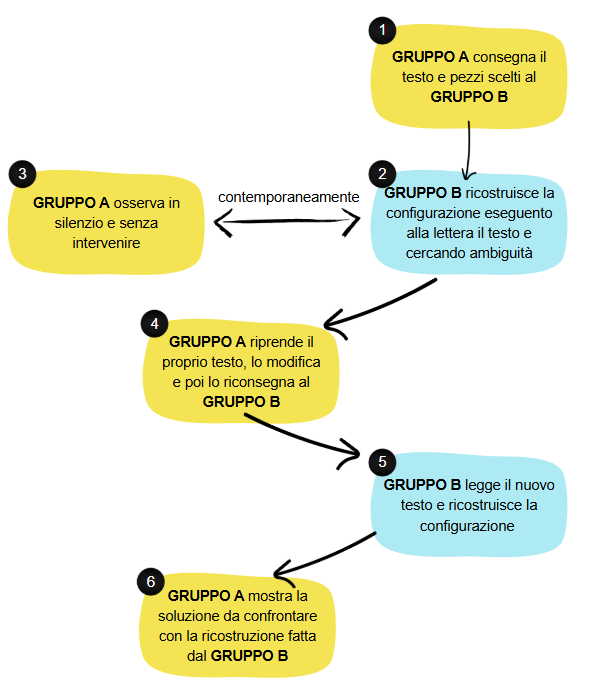
\includegraphics[width=\linewidth]{img/cap3-debug-gruppi.png}\label{credito:debug-luci-originali-1}
\caption{Schema dei passaggi di debugging (Attività 3, Fase 2, Parte 3) tra i due gruppi.}
\label{fig:debug-gruppi}
\end{figure}

\section{Possibili estensioni, variazioni e personalizzazioni }\label{possibili-estensioni-variazioni-e-personalizzazioni}


\subsection{Spunti per adattare le attività}

In caso di difficoltà:


\begin{itemize}
\item
  Diminuire il numero di elementi da gestire (es. il numero di immagini da riordinare o il numero di pezzi a disposizione per creare la configurazione geometrica).
\item
  Invece di chiedere di scrivere dei testi, fornire opzioni di testi già scritti tra cui scegliere quello corretto.
\end{itemize}

Come rendere le attività più sfidanti:

\begin{itemize}
\item
  Aumentare il numero o il tipo di elementi da gestire (ad esempio, nella Fase 2 dell'attività \emph{Descrivere configurazioni geometriche} si può proporre di lavorare su configurazioni tridimensionali).
\item
  Proporre una storia ``sbagliata'' in cui prima individuare le parti principali per poi riordinarle.
\end{itemize}

\section{Aspetti informatici }\label{aspetti-informatici}

In informatica, la sequenza di istruzioni è la struttura di base su cui si costruisce ogni programma. Prima di introdurre strutture più complesse come le selezioni (\emph{se-allora}) o le ripetizioni (\emph{ripeti}), è essenziale che gli alunni e le alunne comprendano a fondo cosa significhi eseguire azioni in un ordine preciso e senza ambiguità.

Queste attività sono particolarmente efficaci perché:

\begin{itemize}
\item
  evidenziano la differenza fra chi crea un programma (programmatore) e chi lo esegue (esecutore);



\item mostrano che un algoritmo deve essere pensato per un esecutore che può eseguire solo un certo insieme di istruzioni ben definito;

\item
  introducono il concetto di debugging come revisione e correzione della sequenza;
\item
  allenano la pianificazione, cioè la capacità di prevedere in anticipo tutti i passi necessari, organizzarli in modo logico e verificarne la completezza.
\end{itemize}

A differenza di una conversazione, in cui è possibile correggere passo-passo ciò che fa l'esecutore, solitamente quando si programma la sequenza viene scritta interamente prima dell'esecuzione\footnote{
  Tralasciamo per il momento forme più interattive di programmazione, che si stanno diffondendo oggi.
  }. Questo richiede un pensiero anticipatorio: occorre immaginare lo svolgimento dell'intero compito, prevedere le criticità e predisporre le istruzioni necessarie a evitarle.

Queste esperienze permettono ad alunni e alunne di esplorare alcune idee chiave:

\begin{itemize}
\item
  \textbf{Ogni azione deve essere descritta in modo esplicito}.
\item
  \textbf{L'ordine conta}: modificare la sequenza può cambiare radicalmente il risultato.
\item
  \textbf{Programmare richiede pianificazione}: occorre pensare prima di agire e prevedere cosa farà l'esecutore.
\item
  \textbf{Le regole condivise} sono indispensabili perché il messaggio sia interpretato nello stesso modo da chi lo scrive e da chi lo legge.
\item
  \textbf{Il debugging è parte del processo}: provare, osservare cosa non funziona, correggere e ripetere.
\end{itemize}

Acquisire familiarità con la sequenza, con la necessità di precisione e con la capacità di pianificare è il primo passo nel percorso di programmazione: solo dopo aver consolidato queste competenze sarà possibile introdurre in modo efficace altre strutture fondamentali come le istruzioni condizionali o le ripetizioni.

\section{Relazione con l'informatica nelle Indicazioni Nazionali 2025 }\label{relazione-con-linformatica-nelle-indicazioni-nazionali}

Relativamente alle Indicazioni Nazionali 2025, queste attività contribuiscono allo sviluppo delle seguenti competenze, obiettivi e conoscenze (queste ultime inserite nelle Indicazioni Nazionali 2025 a titolo di esempio, non prescrittive).


\subsubsection{Competenze (alla fine della scuola primaria) nella disciplina Matematica}


\begin{itemize}
\item
  \emph{Descrivere procedure per lo svolgimento di compiti pratici mediante algoritmi.}
\end{itemize}


\subsubsection{Obiettivi (alla fine della terza primaria) nella disciplina Matematica}


\begin{itemize}
\item
  \emph{Descrivere a parole attività della vita quotidiana tramite sequenze di passi precisi e non ambigui e saperle eseguire.}
\item
  \emph{Scrivere semplici programmi e verificare, mediante la loro esecuzione, se svolgono il compito previsto ed eventualmente correggerli}. Sebbene queste attività siano unplugged (senza computer), si va nella direzione di linguaggi formali con una sintassi e una semantica ben definite e non ambigue. Per questo sono una buona preparazione per questo obiettivo, poiché sono orientate alla progettazione e scrittura di programmi, e alla loro valutazione (controllo di correttezza, debugging, \ldots).

\end{itemize}


\subsubsection{Conoscenze (scuola primaria) nella disciplina Matematica}



\begin{itemize}
\item
  \emph{concetto di algoritmo e sua esecuzione rigorosa};
\item
  \emph{strutture di controllo fondamentali di un linguaggio di programmazione} (In questo capitolo si lavora in particolare sulla sequenza);
\item
  \emph{controllo di correttezza dei programmi}.
\end{itemize}

\section{Valore costruzionista }\label{valore-costruzionista}

Seguendo la prospettiva di Papert, l'apprendimento passa per la costruzione di artefatti significativi di vario tipo che possono essere mostrati, discussi e migliorati insieme. In questo processo, l'errore non è qualcosa da evitare ma è una risorsa, un'informazione preziosa che rende visibili ambiguità e sottintesi e spinge a rendere le istruzioni sempre più chiare. Sequenze ambigue, indicazioni incomplete o termini poco chiari diventano occasioni per riflettere, riformulare e affinare il proprio lavoro attraverso cicli di prova, osservazione e revisione (debugging). La progressione delle attività proposte in questo capitolo - dall'ordinamento di istruzioni fino allo stabilire un linguaggio convenzionale condiviso per \emph{descrivere configurazioni geometriche} - mette in evidenza un approccio tipico in informatica: affrontare la complessità scomponendo i problemi e stabilendo regole condivise che rendano le procedure eseguibili in modo prevedibile. In questo modo alunni e alunne imparano a progettare, verificare e migliorare le proprie soluzioni.

\section{Suggerimenti per ulteriori attività}\label{suggerimenti-per-ulteriori-attivituxe0-e-riferimenti}

Ulteriori attività e riferimenti possono essere reperiti ai seguenti collegamenti.

\printbibliography[heading=none,keyword={cap3},category={attivita}]

\begin{rimandiquaderno}
Se possiedi il volume studente \emph{Sulle orme di Milù -- Informatica}
(Mondadori Education, 2026), puoi usare i rimandi seguenti per affiancarlo
alle attività di questo capitolo.\par\smallskip

\begin{itemize}[leftmargin=*,itemsep=5pt,topsep=4pt]
\item \textbf{Attività 1 -- Sequenze e ordinamenti.} Le attività qui proposte sono analoghe a quelle delle pagine 2 e 3 intitolate RIORDINARE. Nell'attività a pagina 2, sono possibili due ordini (la prima istruzione può essere quella di aprire lo zaino o di prendere i libri).
\item \textbf{Attività 2 -- Istruzioni e programmi.} Le schede ISTRUZIONI E PROGRAMMI (pagg.~4--5) propongono le attività sulla formulazione e sull'esecuzione letterale delle istruzioni: a pag.~4 si trova il panino al cioccolato. Il programma esemplificato nell'Attività 2 della guida è quello della prima attività di pag.~5, rappresentato con blocchi colorati che richiamano i linguaggi visuali, come Scratch.
\item \textbf{Attività 3 -- Descrivere configurazioni geometriche.} Le schede DESCRIVERE UNA FIGURA (pagg.~6--7) si possono usare per preparare o rafforzare le due fasi dell'attività: pag.~6 per la Fase 1 e pag.~7 per la Fase 2. \textbf{Soluzione di pag.~6:} fra Alice e Bob, è Alice a fornire una descrizione che permette di individuare in modo univoco la figura corretta fra le due proposte.
\end{itemize}
\end{rimandiquaderno}
